% Chapter Template

\chapter{Secure Neighbour Discovery Protocols} % Main chapter title

\label{Chapter4} % Change X to a consecutive number; for referencing this chapter elsewhere, use \ref{ChapterX}

\lhead{Chapter 4. \emph{Secure Neighbour Discovery Protocols}} % Change X to a consecutive number; this is for the header on each page - perhaps a shortened title

%----------------------------------------------------------------------------------------
%	SECTION 3
%----------------------------------------------------------------------------------------

We have already presented a set of device pairing protocols and formally analysed them at the previous chapters. Basically, by adapting human assistance, wireless devices can establish secure connections among them. Before this stage, each device, indeed, must know existence of its partners. Certainly, ability to determine the existence of participants within physical range in many systems from cellular infrastructure-based networks, wireless local area network to sensor networks, and short range wireless technologies is fundamental problem. Moreover, security mechanisms for it should be seriously considered. 

One potential threat is that due to different wireless interfaces with different signal power, false results from distance calculation in many neighbour discovery mechanisms might appear. The threat is an old-school problem in traditional wireless networks, but it becomes a serious in distributed systems with heterogeneous devices. Attackers can take advantage to generate false connections, that significantly reduces stability of the systems. This has not mentioned before. 

We put ourselves deeply between these problems, and find that some particular neighbour discovery protocols using time-based, or location-based mechanisms are vulnerable. Meanwhile, current formal verification reasoning about security neighbour discovery protocols cannot resolve the problems. This motivates us to study more secure neighbour discovery mechanisms in context of Internet of Things where a huge amount of heterogeneous devices are interoperating. 

Contributions of this chapter are following:
\begin{enumerate}
\item We present existing neighbour discovery protocols, address their limitations, and present some incorrect existing protocols.  
\item We adapt our formalisation on Strand Spaces with some extensions on physical characteristics and some helpful propositions to deal with statuses of links among principals. 
\item Our model allows us obtain a notable result. We prove that time-based or distance-based neighbour discovery schemes cannot confidentially achieve their goals due to difference of physical signal power of principals. 
\end{enumerate}

Chapter 4 begins with a comprehensive survey of current proposals of neighbour discovery techniques, and vulnerabilities. We then present some incorrect protocols and conduct correct ones. We conduct formalisation based on Strand Space in the next part.  
 
 \section{Overview on Neighbour Discovery Protocols}

<<<<<<< HEAD
To begin with, we introduce a definition of a neighbour discovery protocol (NDP) referred at ~\cite{ndp}:
\begin{Definition}
A neighbour discovery protocol is a protocol that operates in link layer of Internet model. It is responsible for auto-configurating nodes, discovery of other nodes on network, determining link-layer addresses of other nodes, and maintaining reachability information about paths to other active neighbour nodes as well. 
\end{Definition}

For instance, in perfect environment with no obstacle and noise, a device can determine its honest neighbours using flying time measurement. A device, called $A$, broadcasts a greeting message to a potential device, called $B$, then $B$ replies to $A$ quickly after receiving this message. Afterward, when completely observing the feed-back message, $A$ measures the time-of-flight, and multiplies it by signal propagation speed in current medium to obtain the distance. If the distance is lower than a pre-defined threshold, $A$ concludes that $B$ is its neighbour.

Above protocol is definitely insecure in environment with existence of attackers. But, it is so important to be fortified. We state the goal of secure neighbour discovery protocol (or SEND) as follows: 

\begin{Definition}[SEND Goal]
Whenever A declares that B is A’s neighbour after A’s SEND process, B apparently runs the protocol and is a desired neighbour of A. Moreover, both sides are closer than their signal ranges.
\end{Definition}

In this session, we explain why neighbour discovery protocols are vital parts in current systems. Then after presenting their threats and vulnerabilities, we sum up existing approaches in categories.
=======
Neighbour discovery is the process by which a node in a network determines the number and identity of other nodes in its vicinity. In wireless context, neighbours are usually defined as nodes that lie within radio range of each other. Nodes considered as neighbours may cooperate in the performance of various tasks such as communications, sensing, and localisation. For instance, in perfect environment with no obstacle and noise, a device can determine its honest neighbours using flying time measurement. A device, called $A$, broadcasts a greeting message to a potential device, called $B$, then $B$ replies to $A$ quickly after receiving this message. Afterward, when completely observing the feed-back message, $A$ measures the time-of-flight, and multiplies it by signal propagation speed in current medium to obtain the distance. If the distance is lower than a pre-defined threshold, $A$ concludes that $B$ is its neighbour.

However, the discovery process is easily abused by malicious ranging activities of attackers in wireless environments. So, there are many approaches for securely discovering neighbours in wireless network. In this session, we explain why neighbour discovery protocols are vital parts in current systems. Then after presenting their threats and vulnerabilities, we sum up existing secure approaches in categories.
>>>>>>> 3d6cc25ad869467a057daa522b35e3cad82b4604

\subsection{Neighbour Discovery Applications}

NDP is discovered under a form of a principal part of many sensitive applications such as physical authentication, network authentication , routing built-up, and localisation. This classification is referred from ~\cite{Marcinthesis}.

\subsubsection*{Physical Authentication}

In some applications, value of distance between two devices is vital to assess authentication goals. For instance, in Passive Keyless Entry and Start~\cite{waraksa1990passive}, a RFID reader can estimate a travelling message flying time to imply distance to companion tags. Similarly to RFID, NFC technology allows smartphones to communicate with other devices such as speakers, headphones or even other smartphones in very short proximity. As the fact of that, neighbour discovery enables devices to find each other. 

\subsubsection*{Network Authentication}
Wireless network demands devices to be authenticated before they access and communicate with others. For instance, when a telephone is willing to access the Internet via a WLAN access point, it must stay in the signal range of the access point. For that purpose, neighbour discovery is a primary part for wireless communications. 

\subsubsection*{Localisation}

When a device wishes to know its current location, it starts broadcasting messages to close GPS satellites, or close WLAN access points to obtain its location information. However, when GPS or WLAN signal is disabled by noise and obstacles due to weather conditions, tree cover, or surrounding buildings, or walls, neighbours' location information could help. For instance, a car cannot locate itself in a long tunnel, then it derives its own location by asking surrounding cars. Hence, these processes apparently stand on a neighbour discovery protocol.

\subsubsection*{Routing Built-up}

Before using a service in ad-hoc network, each device needs to construct a path from itself to a destination. As always, each device constructs a potential network topology by looking for many or all nodes in the network. According to the current network topology, an appropriate path will be picked up. In fact, exploring neighbours is always a primary step at the beginning. 

\subsection{Threat and Vulnerabilities}\label{threatndp}
Classification of threats and vulnerabilities in neighbour discovery protocols is really paintful due to these following reasons. (i) Attackers could be either legitimate principals or outside intruders, or both. (ii) Some attacks happen across layers from physical layer to network one. 

Therefore, we classify the attacks by two ways. The first way is differentiating internal and external attacks. 

\begin{itemize}
\item \textbf{Internal attacks} are types of attacks where intruders compromise several honest participants. Subsequently, they can imitate all honest behaviours, and intentionally generate fake information. 
\item \textbf{External attacks}, in the contrast, are types of attack where intruders are not capable of compromising honest participants and private information. However, they can overhear, reply, and jam messages. 
\end{itemize}

This way sometime makes confusion in some kinds of attacks such as wormhole, and relay attack where attacker could be both insiders and outsiders. As an alternative way, we consider three specific famous attacks on neighbour discovery protocols: \emph{spoofing attack}, \emph{relay attack}, and \emph{tunneling attack}.

\textbf{Spoofing Attack}: In wireless context, spoofing attack is a situation in which an intruder (i) successfully pretends to be someone else to gain a connection to another participant, or (ii) pretends to own a connection to another participant, but actually does not have. The first type is called identification spoofing, while the second is link spoofing attack. 

\textbf{Relay Attack}: According to observation, relay attack demonstrates a situation where messages are relayed between two honest participants by an intruder. Moreover, we consider two types of relay attack. One is store-and-forward relay where a message is completely received before relayed, while others is fast relay where a message is relayed bit-by-bit. 

\textbf{Tunneling Attack} Tunnelling attack, a special kind of replay attack, happens in a long range distance. Two internal adversarial participants tunnel ND messages so that they appear as neighbours on routes constructed by routing protocols. As a result of that, traffic of some nodes on network probably are controlled by these adversarial nodes. In literature, wormhole attack is another name of tunnelling attack. 

There are also two kinds of tunnelling attack in routing context, one is in-band tunnelling, and the other is out-of-band tunnelling. In-band tunnelling describes that messages are encapsulated at one adversarial node, routed through the network as normal packets, and opened at an adversarial companion. In turn of out-of-band tunnelling, messages are routed in a fast private channel.

\subsection{Neighbour Discovery Techniques}

We classify existing notable techniques of neighbour discovery into six primary categories. Additionally, in references to history, neighbour discovery methods assume that all protocol participants are honest, so internal malicious behaviours are not taken into account. Another speaking, traditional approaches only cope with relay attack and wormhole attack. 

\subsubsection*{Time-based Techniques}

There are two main approaches using time-based techniques: single message-scheme and challenge-respond scheme. 

In single message-schemes as ~\cite{Brands:1994aa,Hancke:2005:RDB:1128018.1128472,Capkun:2003:SST:986858.986862,Yih-ChunHu2002}, each device equipped the same synchronized clock periodically broadcasts greeting authenticated messages including its current timestamp. Thank to precisely synchronized clock, any neighbour device receiving this message easily estimates the distance from itself to the source of the message. 

To overcome clock synchronisation limitations, challenge-response schemes such as in~\cite{4110280},\cite{FaridNait-Abdesselam2008} implemented the RTS/CTS mechanism of IEEE 802.11. 

\subsubsection*{Location-based Techniques}

The neighbour information in proposals~\cite{Yih-ChunHu2002,LOUKASLAZOS,LoukasLazos2005, 4146955} is provided at deployment stage, that allows participants to determine their neighbours' location. An alternative method~\cite{1589106} is using secure localisation schemes in which a device includes its location information in its packets. 

<<<<<<< HEAD
However, the assumptions on trusted location information could be impractical. When an adversary compromises one or more honest devices, it can send counterfeit location information to its neighbours. Hence, combination of timestamps and location in ~\cite{Shokri:2009:PSN:1514274.1514302} can offer better security mechanisms.
=======
However, the assumptions on trusted location information could be impractical. When an attacker compromises one or more honest devices, it can send counterfeit location information to its neighbours. Hence, combination of timestamps and location in ~\cite{Shokri:2009:PSN:1514274.1514302} can offer better security mechanisms.
>>>>>>> 3d6cc25ad869467a057daa522b35e3cad82b4604

\subsubsection*{Device Fingerprinting Techniques}

Complicated techniques using RF signal characteristics allow a device to identify other individual devices. The techniques~ \cite{Kasper, OktayUreten2007, VladimirBrik} are based on the fact that every device with a specific wireless adapter and driver differently generates a different signal pattern. By that way, a sensitive receiver probably identifies the source of signal. More complicated techniques ~\cite{SumanJana, 5211943, 819017} used other variables such as frequency error, SYNC correlation, I/Q offset error to enhance identification accuracy. 

\subsubsection*{Channel Fingerprinting Techniques}

Channel states, presented at~\cite{4289438, LiangXiao2008,LiangXiao2009,Liu:2009:SWC:1823633}, characterized by channel impulse response (CIR) in location-specific, or in time-specific can be used to increase accuracy of detecting source of signal. For instance, a device $A$ will not observe correlated CIR from $B$ when $A$ stands outside the $B$'s RF wavelength apart.

\subsubsection*{Directional Antennas-based Techniques}

Multi-directional antennas used in~\cite{Hu04usingdirectional},~\cite{RuiZhang2010} were applied against worm hole attack. Under assumptions of a disk model, each an antenna spans a specific zone and direction. By this characteristic, when a device sends a message in a specific zone, this message is received in opposite zone of another one. 

\subsubsection*{Connectivity-based Techniques}

Connectivity-based techniques basically can detect changes of muti-hops network when any wormhole is created. Moreover, some approaches tried to identify the wormhole and to remove its effects. Two main methods in the literature are centralised schemes and decentralised schemes. 

In the centralised schemes \cite{RuiZhang2010},~\cite{WeichaoWang2007}, visualisation of connectivity graph of the network constructed from coordinates of devices for multi-scaling dimension can be monitored either manually by human operator or automatically by software to detect and localise the wormhole. 

In decentralised schemes, k-hops neighbour information used in~\cite{RiteshMaheshwari}\cite{4699583} were considered as local connectivity to detect and remove a false link in network. Some alternative methods~\cite{RiteshMaheshwari} and ~\cite{5993472} used features generalised edge-clustering coefficient to eliminate connectivity model.

\section{Vulnerabilites of Exisiting Protocols}

This section presents some notable flaws in some famous protocols. The problem in~\cite{Brands:1994aa} was introduced at ~\cite{6234408}, while the other one was found in~\cite{lin2006}. 

\subsection{Brands \& Chaum Protocol Vunerabilities}

Brands \& Chaum(BC) protocol \cite{Brands:1994aa}, the famous distance bounding protocol, enables a verifier to properly estimate the physical distance to its authenticated prover. The protocol works as follows.
\begin{enumerate}
\item Both sides generate their own random number, then rapidly exchanges bit-by-bit to together.
\item The verifier sends a message consisting of the two random numbers, and its signature to the verifier. 
\item The verifier verifies the distance, random values, and the prover's identity in order to accept the connection
\end{enumerate}

To simplify the protocol, we consider the rapid bit-exchange channel as a short-range public out-of-band channel for transmitting random values. The protocol is described below. 

\begin{center}
\begin{flushleft}
 \emph{M1}: $A \rightarrow B :\{A,B\}$ \\
\emph{M2}: $[B \rightarrow A]_o :\{N_B\}$ \\
\emph{M3}: $[A \rightarrow B]_o : \{N_A\}$\\
<<<<<<< HEAD
\emph{M4}: $B \rightarrow A :\{N_A \otimes N_B\}$ \\
=======
\emph{M4}: $B \rightarrow A :\{N_A \oplus N_B\}$ \\
<<<<<<< HEAD
\emph{M5}: $B \rightarrow A : \{|N_A,N_B|\}_{KB}$
=======
>>>>>>> leneutre/master
\emph{M5}: $B \rightarrow A : \{N_A,N_B\}_{KB}$
>>>>>>> 3d6cc25ad869467a057daa522b35e3cad82b4604
\end{flushleft}
\end{center}

To violate the SEND goal, attacker $P$ must make a device $A$ to accept him as the prover. Moreover, the authors did not cover the attack where a distant party with a secret key cooperates with a close party (without conveying secret keys) to complete a protocol. As a result, discovered in the paper~\cite{6234408}, a flaw exploits at the last phase by using an advantage of a high power antenna. The attack scenario is presented at figure~\ref{fig:hijacking_case}. 

\begin{figure}
	  \caption{BC Protocol Attack}\label{fig:hijacking_case}
	  \centering
 		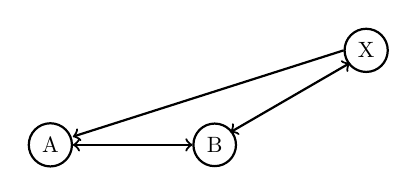
\begin{tikzpicture}[thick,scale=0.8, every node/.style={scale=0.8}]
		\draw [<->](1,1) node[anchor=east,circle,draw]{A} to (2.9,1) node[anchor=west,circle,draw]{B};
		\draw [<-](1,1.13) to (5.3,2.5) node[anchor=west,circle,draw]{X};
		\draw [<->](3.5,1.2) to (5.4,2.3);
	    \end{tikzpicture}
		
		\begin{tikzpicture}[implies/.style={double,double equal sign distance,-implies},
  			 dot/.style={shape=circle,fill=black,minimum size=2pt,
             inner sep=0pt,outer sep=2pt},thick,scale=0.8, every node/.style={scale=0.8}]
		\matrix[matrix of nodes] {
  		|[dot,label=above:$A$] (A1)| {} & [2cm] |[dot,label=above:$B$] (B1)| {} & [2cm]|[label=above:$X$] (X1)| {}\\[1cm]
  		 |[dot] (A2)| {} & [2cm] |[dot] (B2)| {} & [2cm]|[] (X2)| {}\\[1cm]
	     |[dot] (A3)| {} & [2cm] |[dot] (B3)| {} & [2cm]|[] (X3)| {}\\[1cm]
		|[dot] (A4)| {} & [2cm] |[dot] (B4)| {} & [2cm]|[] (X4)| {}\\[1cm]
  		 |[dot] (A5)| {} & [2cm] |[] (B5)| {} & [2cm]|[dot] (X5)| {}\\[1cm]
 		 |[] (A6)| {} & [2cm] |[dot] (B6)| {} & [2cm]|[dot] (X6)| {}\\[1cm]
 		 |[dot] (A7)| {} & [2cm] |[] (B7)| {} & [2cm]|[dot] (X7)| {}\\[1cm] };
	
		\draw (A1) edge[->] node[above] {M1} (B1)
	      edge[implies] (A2); 
		\draw [-latex,densely dotted](B2) edge[->] node[above] {M2} (A2);
	     \draw (A2) edge[implies] (A3);
		\draw [-latex,densely dotted](A3) edge[->] node[above] {M3} (B3);
    	  \draw (B1) edge[implies] (B2);
		\draw (B4) edge[->] node[above] {M4} (A4)
    	  edge[implies,implies-] (B3);
		\draw (B2) edge[implies] (B3);
		\draw (A3) edge[implies] (A4);
		\draw (A4) edge[implies] (A5);
		\draw (B4) edge[implies] (B6);
		\draw [-latex,densely dashed](X5) edge[->] node[above] {MR} (A5);
		\draw (B6) edge[->] node[above] {M5} (X6);
		\draw (X5) edge[implies] (X6);
		\draw (X7) edge[->] node[above] {M5'} (A7);
		\draw (B5) edge[implies] (B6);
		\draw (X6) edge[implies] (X7);
		\draw (A5) edge[implies] (A7);
		\end{tikzpicture} 

\end{figure}

\subsection{ADVSIG Vulnerability}

<<<<<<< HEAD
ADVSIG proposed by INRIA group~\cite{Raffo:2004:ASS:1029102.1029106} is a kind of secure routing protocol fortifying for OLSR \cite{Clausen:2003:OLS:RFC3626}. In this protocol, a node wishes to detect neighbour nodes with a direct and bi-directional link. Any link must be checked to be considered validation. We realise that compared to OLSR specification, third message of ADVSIG changed SYMMETRIC LINK status to ASYMMETRIC LINK status. This change may affect to neighbours of A if no new message from A informs that A owns a symmetrical link A to B. The protocol is presented as below. 
\begin{flushleft}
 \emph{M1:} $A \to [B]: \{|\O, \O, t_0|\}_{KA}$\\
 \emph{M2:} $B \to [A]: \{|\{|"A:ASYM\_LINK", t_1|\}_{KB}, \O,t_1|\}_{KB}$\\
\emph{M3:} $A \to [B]: \{|\{|"B:ASYM\_LINK",t_2|\}_{KA},\O ,t_2 |\}_{KA})$\\
 \emph{M4:} $B \to [A] : \{|\{|"A:SYM\_LINK", t_3|\}_{KB} ,\{|"B:ASYM\_LINK",t_2|\}_{KA} ,t_3|\}_{KB})$
=======
ADVSIG proposed by INRIA group~\cite{Raffo:2004:ASS:1029102.1029106} is a kind of secure routing protocol fortifying for OLSR \cite{Clausen:2003:OLS:RFC3626}. In this protocol, a node wishes to detect neighbour nodes with a direct and bi-directional link. Any link must be checked to be considered validation. We realise that compared to OLSR specification, third message of ADVSIG changed SYMMETRIC LINK status to ASYMMETRIC LINK status. This change may affect to neighbours of A if no new message from A informs that A owns a bidirectional link A to B. The protocol is presented as below. 
\begin{flushleft}
 \emph{M1:} $A \to [B]: \{\O, \O, \tau_0\}_{KA}$\\
 \emph{M2:} $B \to [A]: \{\{"A:ASYM\_LINK", \tau_1\}_{KB}, \O,\tau_1\}_{KB}$\\
\emph{M3:} $A \to [B]: \{\{"B:ASYM\_LINK",\tau_2\}_{KA},\O ,\tau_2 \}_{KA})$\\
 \emph{M4:} $B \to [A] : \{\{"A:SYM\_LINK", \tau_3\}_{KB} ,\{"B:ASYM\_LINK",\tau_2\}_{KA} ,\tau_3|\}_{KB})$
>>>>>>> 3d6cc25ad869467a057daa522b35e3cad82b4604
\end{flushleft}

Moreover, every valid link state must satisfy a maximum interval $\delta_{max}$ defined by $|T_{Sender} - T_e | < \delta_{max}$ where $T_{Sender}$ is the value clock of the sender, and $T_e$ is the value clock of receiver. 

<<<<<<< HEAD
Provided that the third message does not include the proof from the second one, Responder cannot ensure if Initiator has been received the second message or not. As the result of that, internal attackers can produce the first and third messages to valid a protocol run with Responder. Additionally,  neighbours of Responder could be impacted by this attack due to two-hop sensing mechanism in the OLSR protocol.  Figure~\ref{advsigattack3} outlines an attacking scenario to ADVSIG where there only appears an asymmetric link X $\rightarrow$ B.
=======
Provided that the third message does not include the proof from the second one, Responder cannot ensure if Initiator has been received the second message or not. As the result of that, internal attackers can produce the first and third messages to valid a protocol run with Responder. Additionally,  neighbours of Responder could be impacted by this attack due to two-hop sensing mechanism in the OLSR protocol.  Figure~\ref{advsigattack3} outlines an attacking scenario to ADVSIG where there only appears an unidirectional link X $\rightarrow$ B.
>>>>>>> 3d6cc25ad869467a057daa522b35e3cad82b4604

\begin{figure}
		\caption{ADVSIG Attack }\label{advsigattack3}
        \centering
        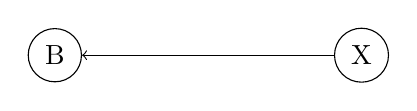
\begin{tikzpicture}
		\draw [<-](1,1) node[anchor=east,circle,draw]{B} to (4.2,1) node[anchor=west,circle,draw]{X};
		\end{tikzpicture}

	    \centering
        \begin{tikzpicture}[implies/.style={double,double equal sign distance,-implies},
  			dot/.style={shape=circle,fill=black,minimum size=2pt,
  		      inner sep=0pt,outer sep=2pt},thick,scale=0.8, every node/.style={scale=0.8}]
		\matrix[matrix of nodes] {
		  |[dot,label=above:$B$] (B1)| {} & [2cm]|[] (C1)| {}&[1cm] |[dot,label=above:$X$] (X1)| {}\\[1cm]
  		  |[dot] (B2)| {} & [2cm]|[dot,label=above:$*$] (C2)| {}& [1cm]|[dot] (X2)| {}\\[1cm]
  	      |[dot] (B3)| {} & [2cm]|[] (C3)| {}& [2cm]|[dot] (X3)| {}\\[1cm]
 		  |[dot] (B4)| {} & [2cm]|[dot,label=above:$*$] (C4)| {}& [1cm]|[] (X4)| {}\\
		};
		\draw (X1) edge[->] node[above] {M1} (B1)
	      edge[implies] (X3); 
		\draw (B2) edge[->] node[above] {M2} (C2)
	      edge[implies,implies-] (B1);
		\draw (B3) edge[<-] node[above] {M3} (X3)
    	  edge[implies,implies-] (B2);
		\draw (B4) edge[->] node[above] {M4} (C4)
    	  edge[implies,implies-] (B3);
		\end{tikzpicture}

\end{figure}

We found the same problem in the work~\cite{Adnane20131159}. Authors proposed a trusted-based security for OLSR protocols where all participants must trust together. However, internal attackers can successfully create a fake bidirectional link to a target as they do in ADVSIG. 

\subsection{Correctness of ADVSIG}
In this part, we would like to propose a simple correctness of ADVSIG scheme. We attach link proofs for the second and the third message. Thus, the first link proof in the second message is a hash of the first message encrypted by B's public key, while the second link proof in the third message is the link state of the previous one. 

<<<<<<< HEAD
$A$'s signature wrapped by hash function is impossible to be reproduced by any adversary. As the result of that, even the adversary incidentally receives the message of $B$, he cannot create a correct reply. An important note that, after the third message, $A$ fully indicates $B$ be its neighbour. For that reason, physical link guaranty must be done before this step. The scheme is presented as follows. 

\begin{flushleft}
 \emph{M1:} $A \to [B]: \{|\O, \O, t_0|\}_{KA}$\\
 \emph{M2:} $B \to [A]: \{|\{|"A:ASYM\_LINK", t_1|\}_{KB},$ $h(\{|\{|\O, \O, t_0|\}_{KA}|\}pub(B)),t_1|\}_{KB}$\\
\emph{M3:} $A \to [B]: \{|\{| "B:SYM\_LINK",t_2|\}_{KA},$ $\{|"A:ASYM\_LINK", t_1|\}_{KB},t_2 |\}_{KA}$\\
 \emph{M4:} $B \to [A] : \{|\{| "A:SYM\_LINK", t_3|\}_{KB},$ $\{| "B:SYM\_LINK",t_2|\}_{KA} ,t_3|\}_{KB}$
=======
$A$'s signature wrapped by hash function is impossible to be reproduced by any attacker. As the result of that, even the attacker incidentally receives the message of $B$, he cannot create a correct reply. An important note that, after the third message, $A$ fully indicates $B$ be its neighbour. For that reason, physical link guaranty must be done before this step. The scheme is presented as follows. 

\begin{flushleft}
 \emph{M1:} $A \to [B]: \{\O, \O, \tau_0|\}_{KA}$\\
 \emph{M2:} $B \to [A]: \{\{"A:ASYM\_LINK", \tau_1\}_{KB},$ $h(\{\{\O, \O, \tau_0\}_{KA}\}pub(B)),\tau_1\}_{KB}$\\
\emph{M3:} $A \to [B]: \{\{ "B:SYM\_LINK",\tau_2\}_{KA},$ $\{"A:ASYM\_LINK", \tau_1\}_{KB},\tau_2\}_{KA}$\\
 \emph{M4:} $B \to [A] : \{\{ "A:SYM\_LINK", \tau_3\}_{KB},$ $\{"B:SYM\_LINK",\tau_2\}_{KA} ,\tau_3\}_{KB}$
>>>>>>> 3d6cc25ad869467a057daa522b35e3cad82b4604
\end{flushleft}

Now, by proofs, A and B easily verify physical bidirectional links between them. 

\section{Formal Analysis of Neighbour Discovery Protocol}

%The problems in some neighbour discovery protocols introduced in previous section question why they had not discovered when the protocols were being constructed and tested. An expensive answer we say is that they have not exhaustedly analysed in formal methods. Additionally, current formal models are not ready for this problem due to strong assumptions on characteristic of physical wireless interfaces, and attackers' capabilities.   

%To tackle this problem, we construct our formalisation based on Strand Spaces theory. In our formalisation, each event is facilitated with timestamps, location information and signal power, so this allows us to formalise neighbour discovery protocols and to discover the problems we presented in the Introduction section. To begin with, we recap existing models and spot their limitations. 

Due to lack of place, we do not recall here the whole theory of Strand Spaces, but focus on the extensions necessary to examine secure neighbour discovery protocol. For a complete background on Strand Spaces the reader can consult~\cite{674832},~\cite{Guttman:2002:ATS:568264.568267}. The extensions mainly concern the physical notations and the penetrator model...
 
Before presenting our model extensions of Strand Spaces, we formulate some supplementary assumptions concerning physical characteristics of wireless interfaces and environment, that we will have to take into account. 

\subsection{Related Work}

Most current approaches formalised time as timestamps to determine key-expiration \cite{Li:2007:ESS:1338438.1338469} , and integrity of messages via round trip time-of-flight ~\cite{Poturalski:2008:TPS:1456396.1456400, RaphaelJamet}. Meanwhile, location information was considered in problems of correctness of routing protocols~\cite{5230621,Basin:2009:LGP:1616077.1616079}, or evaluating distance between two neighbours in \cite{Poturalski:2008:TPS:1456396.1456400}. Barely found in literature, signal characteristic is an interesting feature mentioned in \cite{Poturalski:2008:TPS:1456396.1456400}. However, this feature is not truly helpful to reveal attacking location and direction. 

Close to our approach, the models~\cite{Yang03modelingvulnerabilities, 4481351} extended Strand Spaces to pick up vulnerabilities in ad-hoc routing protocols while other approaches \cite{Li:2007:ESS:1338438.1338469, Sharp:2007:TTS:2391910.2391948} expressed temporal phenomena, and notably key-expiration. In addition to, metric strand proposed in \cite{Thayer:2010aa} was presented to deal with locale authentication. Nevertheless, no specified attack and proof was provided in this work. 

\subsection{Assumptions}

We explicitly declare some reasonable assumptions as follows:
\begin{itemize}
\item Every participant is equipped with: (I) \textit{various types of wireless devices with different signal powers}, (ii) \textit{precise clock devices}. To make simplicity, radiation power is assumed to stay the same during protocol execution.
\item An \textit{idealized communication environment} is regarded where wireless signal travels on non-obstacle path with speed of light \emph{c}. Following this assumption, when a participant stands on signal propagation region of others, he can listen to their exchanged messages. 
\item A \textit{secure key distribution function} is enabled on all participants. 
\end{itemize}

Furthermore, our current work only focuses on \textit{a static wireless network model} where objects do not change their position due to complexity of modelling dynamic networks. Dynamic network, hence, could be extended and considered in our future work. 

\subsection{Wireless Strand Spaces}

<<<<<<< HEAD
Actually, original Strand Spaces was designed for cryptographic protocols, so it apparently cannot deal with neighbour discovery protocols. To tackle this limitation, we facilitate Strand Spaces model with our extensions to account for wireless context, then we call the \textit{wireless Strand Spaces}. In particular, a node in our model is equipped with \textit{location, timestamp, signal range} values. Location shows where the node is standing, timestamp indicates when a node happens, and signal range refers to how far the wireless signal of the node can reach. As consequence, the definition of a wireless node is presented as belows.

\begin{Definition}[Wireless Node] A \emph{wireless node} $n$ is a tuple of $(t, l_n, t_n, R_n)$ where $t$ is a signed term, $l_n$ is location, $t_n$ is a timestamp, and $R_n$ is signal range.\end{Definition}

Note that, $l_n$, \textit{location of a node n}, is extensible to any Euclidean space. \textit{Distance between nodes} $n$ and $n'$ is noted $dist(l_n,l_n')$ or $dist(n,n')$. \textit{Timestamp}, $t_n$, appears in a node to check freshness property, and it is a value of local clock when an event begins. \textit{Signal range of a node n}, $R_n$, is a positive real number. 
=======

Obviously, original Strand Spaces was designed for cryptographic protocols, so it apparently cannot deal with neighbour discovery protocols. To tackle this limitation, we facilitate Strand Spaces model with our extensions to account for wireless context, then we call the \textit{wireless Strand Spaces}. In particular, a node in our model is equipped with \textit{location, timestamp, signal range} values. Location shows where the node is standing, timestamp indicates when a node happens, and signal range refers to how far the wireless signal of the node can reach. As consequence, the definition of a wireless node is presented as below.

\begin{Definition}[Wireless Node] A \emph{wireless node} $n$ is a tuple of $(t, l_n, \tau_{n}, R_n)$ where $t$ is a signed term, $l_n$ is location, $\tau_{n}$ is a timestamp, and $R_n$ is signal range.\end{Definition}

Note that, $l_n$, \textit{location of a node n}, is extensible to any Euclidean space. \textit{Distance between nodes} $n$ and $n'$ is noted as $dist(n,n')$. \textit{Timestamp}, $\tau_{n}$, appears in a node to check freshness property, and it is a value of local clock when an event begins. \textit{Signal range of a node n}, $R_n$, is a positive real number. According to assumption~\ref{assum}, signal power does not change during a protocol execution; hence, we denote $R_{st}$ is physical signal  propagation of strand $st$. 
>>>>>>> 3d6cc25ad869467a057daa522b35e3cad82b4604

In realistic scenarios, there always exists a gap between two events, so a fixed value $\delta_{tp}$ is noted as a \textit{processing delay} of edge $ (+n) \Rightarrow (-n')$. We continue describing definitions of wireless strand, and wireless bundle. 

\begin{Definition}[Wireless Strand] A \emph{wireless strand} is a strand with wireless nodes.
\end{Definition}

<<<<<<< HEAD
Recall that static network is being discussed in this article; hence, a strand with fixed location is so-called \textit{a fixed wireless strand}. Thus, all nodes in a fixed strand share the same location. To avoid ambitious notions, notion of strand in this section is now refer to a wireless strand. 

In our extension, we need to explicitly distinguish between different types of links. A link is a generic term denoted a relationship between two participants. There are two kinds of links: \emph{logical} and \emph{physical}. While a logical link describes existence of path of a term from one strand to another, a physical one describes a directional and physical path without any relaying point from one strand to another one. Moreover, each type of link has two states: \emph{single} and \emph{double}. A single link means an unidirectional connection when a double link means a bidirectional one. 

Actually, existence of a physical link is usually hard to be correctly criticised due to environment complexity. Hence, in this work, a physical link is simply evaluated by a distance value among participants. Precisely speaking, by any mean, a double physical link exists between two participants if and only if the distance between them is lower than their own signal coverage. Thus, we formally define notations of links as follows.

\begin{Definition}
\begin{itemize}
\item \emph{Single physical link}: $\forall st,st' \in \mathcal{B}$, $plink(st,st', \rightarrow) \Leftrightarrow$ $dist(st,st') \le R_{st}$.
\item \emph{Double physical link}: $\forall st,st' \in \mathcal{B}$, $plink(st,st', \leftrightarrow) \Leftrightarrow$ $(dist(st,st') \le R_{st}) \wedge (dist(st',st) \le R_{st'})$.
\item \emph{Single logical link}: $\forall st, st' \in \mathcal{B}, n \in st, n' \in st', \exists (n_1 \rightarrow^* n_2) \Leftrightarrow \exists link(st, st',\rightarrow)$.
\item \emph{Double logical link}: $\forall st, st' \in \mathcal{B},$ $ \exists link(st, st',\rightarrow) \wedge \exists link(st', st,\rightarrow) \Leftrightarrow \exists link(st, st',\leftrightarrow)$.
=======
Recall that static network is being discussed in this article; hence, a strand with fixed location is so-called \textit{a fixed wireless strand}. Thus, all nodes in a fixed strand share the same location. We denote $loc(st)$ be the location of strand $st$, and $dist(st,st')$ be the distance between two strand $st$ and $st'$. To avoid ambitious notions, notion of strand in this section is now refer to a wireless strand. 

In our extension, we need to explicitly distinguish between different types of links. A link is a generic term denoted a relationship between two participants. There are two kinds of links: \emph{logical} and \emph{physical}. While a logical link describes existence of path of a term from one strand to another, a physical one describes a directional and physical path without any relaying point from one strand to another one. Moreover, each type of link has two states: \emph{unidirectional} and \emph{bidirectional}. 

Existence of a physical link is usually hard to be precisely criticised due to environment complexity. Hence, in this work, a physical link is simply evaluated by a distance value among participants. Another speaking, by any mean, a bidirectional physical link exists between two participants if and only if the distance between them is lower than their own signal coverage. We formally define notations of links as follows.

\begin{Definition}
\begin{itemize}
\item \emph{Unidirectional physical link}: $\forall st,st' \in \mathcal{B}$, $plink(st,st', \rightharpoonup) \Leftrightarrow$ $dist(st,st') \le R_{st}$.
\item \emph{Bidirectional physical link}: $\forall st,st' \in \mathcal{B}$, $plink(st,st', \rightleftharpoons) \Leftrightarrow$ $(dist(st,st') \le R_{st}) \wedge (dist(st',st) \le R_{st'})$.
\item \emph{Unidirectional logical link}: $\forall st, st' \in \mathcal{B}, n \in st, n' \in st', \exists (n_1 \rightarrow^* n_2) \Leftrightarrow \exists link(st, st',\rightharpoonup)$.
\item \emph{Bidirectional logical link}: $\forall st, st' \in \mathcal{B},$ $ \exists link(st, st',\rightharpoonup) \wedge \exists link(st', st,\rightharpoonup) \Leftrightarrow \exists link(st, st',\rightleftharpoons)$.
>>>>>>> 3d6cc25ad869467a057daa522b35e3cad82b4604
\end{itemize}	
\end{Definition}

\subsection{Extended Penetrator Model}\label{penndp2}

<<<<<<< HEAD
Relaying attack and link spoofing attack are two serious malicious events against neighbour discovery goals. \textbf{Spoofing attack} is a situation in which an intruder (i) successfully pretends to be someone else to gain a connection to another participant, or (ii) pretends to own a connection to another participant, but actually does not have. According to observation, \textbf{relay attack} demonstrates a situation where messages are relayed between two honest participants by an intruder. 

These attacks are apparently conducted from a sequence of atomic events such as sending events with high a power antenna  and single replaying events respectively. Hence, we encode the atomic malicious actions into two new penetrator strands. Precisely, given penetrator strand $s_p$, and $n, n' \in s_p$. 
\begin{itemize}
\item[SR.] \emph{Single relay:} \\ $\langle -(t, l_n, t_n, R_n), +(t, l_n', t_{n'}, R_{n'}) \rangle >$ where $t_{n'} - t_n = 0$.
\item [BS.] \emph{Boosting signal:} $\langle +(t, l_n, t_n, R_M) \rangle$ where $R_M$ could be an unlimited value. 
\end{itemize}

At present, single relaying attack is possibly detected by advanced protection mechanisms presented in the previous section. Therefore, we consider the \emph{weak penetrator model} be a model which does not deal with relaying attack. In contrast, \emph{strong penetrator model} has full attacker's capabilities. 

\subsection{Modeling Goals}

We express this goal in Strand Spaces model as an authentication goal:

\emph{Secure Neighbour Disovery Goal:} \textit{For all bundles $\mathcal{B}$, two roles $R, R' \in \mathcal{B}$, and all strand $st$, there exists a strand $st$' such that if $st \in R$ has $ \mathcal{B}_{height}$ i and some protocol assumptions hold then $st' \in R'$ has $\mathcal{B}_{height}$ j and there exists a physical link $plink(st,st',\leftrightarrow)$.}
=======
Along with Dolev-Yao penetrator model~\cite{dolev-yao}, this article considers two physical attacks: relaying attack and link spoofing attack since they are two serious malicious events against neighbour discovery goals. \textbf{Spoofing attack} is a situation in which an intruder (i) successfully pretends to be someone else to gain a connection to another participant, or (ii) pretends to own a connection to another participant, but actually does not have. According to observation, \textbf{relay attack} demonstrates a situation where messages are relayed between two honest participants by an intruder. 

These attacks are apparently conducted from a sequence of atomic events such as sending events with high a power antenna  and single replaying events respectively. Hence, we encode the atomic malicious actions into two new penetrator strands. Precisely, given penetrator strand $s_p$, and $n, n' \in s_p$. 
\begin{itemize}
\item[SR.] \emph{Single relay:} \\ $\langle -(t, l_n, \tau_{n}, R_n), +(t, l_n', \tau_{n'}, R_{n'}) \rangle >$ where $\tau_{n'} - \tau_{n} = 0$.
\item [BS.] \emph{Boosting signal:} $\langle +(t, l_n, \tau_{n}, R_M) \rangle$ where $R_M$ could be an unlimited value. 
\end{itemize}

At present, single relaying attack is possibly detected by advanced protection mechanisms presented in the previous section. Therefore, we consider the \emph{weak penetrator model} be a model which does not deal with relaying attack. In contrast, \emph{strong penetrator model} has full attacker's capabilities. 
We express this goal in Strand Spaces model as an authentication goal:

\emph{Secure Neighbour Disovery Goal:} \textit{For all bundles $\mathcal{B}$, two roles $R, R' \in \mathcal{B}$, and all strand $st$, there exists a strand $st$' such that if $st \in R$ has $ \mathcal{B}_{height}$ i and some protocol assumptions hold then $st' \in R'$ has $\mathcal{B}_{height}$ j and there exists a physical link $plink(st,st',\rightleftharpoons)$.}
>>>>>>> 3d6cc25ad869467a057daa522b35e3cad82b4604

Guttman stated that analysing authentication properties of a protocol means finding right choices for $R$ and $R'$ for $i$, and $j$, and necessary origination assumptions. However, this proving way could extremely cost time and effort when solving a complicated protocol. So, to ease this job, Guttman introduced authentication tests~\cite{authenticationtests} as supporting tools. Following to this idea, we construct our authentication link tests to guarantee whether a protocol satisfies the goal or not.  At first, we introduce a link test edge, and an authentication logical link test. Then, we conduct authentication physical link tests based on time and location estimation. 

\subsection{Logical Link Tests}

<<<<<<< HEAD
To get rid of link spoofing attack, a protocol should support a mechanism to enable a participant to verify whether his protocol-mate has already seen its messages or not. As a solution, challenge-respond mechanisms, described formally as authentication tests, could be used in which a participant delivers a random as a challenge and receives an answer only produced by an intended sender. The answer usually contains a cryptographic part as a proof that allows the participant verifies origin, integrity, or confidentiality of this message. 

One possible particular proof, called \textit{hidden proof}, is a nonce encrypted by pre-shared key, or a nonce encrypted by public key of Initiator, or a hash of nonce and name of Responder. Another one, called \textit{clear proof}, is a part of previous Initiator's message that contains Responder's ID and a timestamp, and is signed by private key of the Initiator. We define notations of \emph{identification factor}, and a \emph{provable component} to express these such proofs. 

\begin{Definition} \emph{An identification factor} in a component $\{|h|\}_K$ is:
\begin{itemize}
	\item(clear-form) \emph{responder's $ID_{Res}$ and a timestamp t} such that $(ID_{Res} \sqsubseteq \{|h|\}_K ) \wedge (t \sqsubseteq \{|h|\}_K$ in which $K$ is a private key of the initiator, or a signature $sig(K)$ encrypted with a private key of the initiator $K$. Or, 
	\item(hidden-form) \emph{a nonce N} such that N $\sqsubseteq \{|h|\}_K$ in which $K$ is a pre-shared secret key or public key of the responder.\end{itemize}
=======
To get rid of link spoofing attack, a protocol should support a mechanism enabling a participant to verify whether his protocol-mate has already seen its messages or not. As a solution, challenge-respond mechanisms, described formally as authentication tests, could be used in which a participant delivers a random as a challenge and receives an answer only produced by an intended sender. The answer usually contains a cryptographic part as a proof that allows the participant verifies origin, integrity, or confidentiality of this message. 

One possible particular proof, called \textit{hidden proof}, is a nonce encrypted by pre-shared key, or a nonce encrypted by public key of Initiator, or a hash of nonce and name of Responder. Another one, called \textit{clear proof}, is a part of previous Initiator's message that contains Responder's ID and a timestamp, and is signed by private key of the Initiator. We define notations of \emph{identification factor}, and a \emph{provable component} to express these such proofs. 

\begin{Definition} \emph{An identification factor} in a component $\{h\}_K$ is:
\begin{itemize}
	\item(clear-form) \emph{responder's $ID_{Res}$ and a timestamp t} such that $(ID_{Res} \sqsubseteq \{h\}_K ) \wedge (t \sqsubseteq \{h\}_K$ in which $K$ is a private key of the initiator. Or, 
	\item(hidden-form) \emph{a nonce N} such that N $\sqsubseteq \{h\}_K$ in which $K$ is a pre-shared secret key or public key of the responder.\end{itemize}
>>>>>>> 3d6cc25ad869467a057daa522b35e3cad82b4604
\end{Definition}

\begin{Definition}\emph{A provable component} is a component which has one of forms:
\begin{itemize}
<<<<<<< HEAD
	\item (clear-form):$\{|m|\}_{Pr(Res)}$ in which $idf \sqsubseteq \{|h|\}_{Pb(Init)} \sqsubseteq m$ where $Pr(Res)$ is a private key of Responder, and $Pb(Init)$ is the public key of Initiator;  
	\item (hidden-from):$\{|m|\}_K$ or $\{hash(m)\}_{Pr(Res)}$ in which $idf \sqsubseteq m$, and K is a pre-shared key, and $Pr(Res)$ is a public key of Responder;
=======
	\item (clear-form):$\{m\}_{Pr(Res)}$ in which $idf \sqsubseteq \{h\}_{Pb(Init)} \sqsubseteq m$ where $Pr(Res)$ is a private key of Responder, and $Pb(Init)$ is the public key of Initiator;  
	\item (hidden-from):$\{m\}_K$ or $\{hash(m)\}_{Pr(Res)}$ in which $idf \sqsubseteq m$, and K is a pre-shared key, and $Pr(Res)$ is a public key of Responder;
>>>>>>> 3d6cc25ad869467a057daa522b35e3cad82b4604
\end{itemize}
\end{Definition}

We conduct \emph{a logical link test}, and \emph{an authentication logical link test} which allows a participant to ensure that none of it's partners completes a protocol run without receiving its messages. We would like to revise the definition of \emph{a test} defined in~\cite{authenticationtests}. 

\begin{Definition}[A Test] 
<<<<<<< HEAD
$t = \{|m|\}_K$ is \emph{a test} for $a$ in $n$ if:
=======
$t = \{m\}_K$ is \emph{a test} for $a$ in $n$ if:
>>>>>>> 3d6cc25ad869467a057daa522b35e3cad82b4604
\begin{enumerate}
\item $a\sqsubseteq t$ and $t$ is a component of $n$;
\item The term $t$ is not a proper subterm of a component of any regular node $n' \in \Sigma$. 
\end{enumerate}
The edge $n \Rightarrow^+ n'$ is \emph{a test} for $a$ if $a$ uniquely originates at $n$ and $n \Rightarrow^+ n'$ is a transformed edge for $a$. 
\end{Definition}

<<<<<<< HEAD
\begin{Definition}[Logical Link Test] The edge $n \Rightarrow^+ n'$ is a \emph{logical link test} for an identification factor $idf$ in $t = \{|m|\}_K \sqsubseteq term(n')$ if it is a test for $idf$ in which $K \not\in P$ and $t$ is a provable component for $idf$ in $n'$
\end{Definition}

The authentication logical link test below results a double logical link between two strands $st$ and $st'$ in a bundle. 
=======
\begin{Definition}[Logical Link Test] The edge $n \Rightarrow^+ n'$ is a \emph{logical link test} for an identification factor $idf$ in $t = \{m\}_K \sqsubseteq term(n')$ if it is a test for $idf$ in which $K \not\in P$ and $t$ is a provable component for $idf$ in $n'$
\end{Definition}

The authentication logical link test below results a bidirectional logical link between two strands $st$ and $st'$ in a bundle. 
>>>>>>> 3d6cc25ad869467a057daa522b35e3cad82b4604
\begin{Proposition}[Authentication Logical Link Test]\label{logicaltest}Let $n \Rightarrow^+ n' \in st$ be a logical link test for an identification factor $idf \sqsubseteq t' \sqsubseteq term(n')$. There exist regular nodes $m, m' \in st'$ such that $t'$ is a provable component of $m'$, and $m \Rightarrow^+ m'$ is a transforming edge for $idf$. 
\end{Proposition}

\begin{proof}
<<<<<<< HEAD
Reusing the proof of proposition 20 in \cite{Guttman:2002:ATS:568264.568267}, we obtain regular edge $m \Rightarrow m'$ in a regular $st'$. On one hand, identification factor $idf$ allows $st'$ to ensure the existence of $st$ in the protocol. On the other hand, a new provable component as well helps $st$ ensure $st'$ has already received the challenge message. As a result, Initiator can ensure existence of a double logical link $link(st,st',\leftrightarrow)$ with Responder. 
=======
Reusing the proof of proposition 20 in \cite{Guttman:2002:ATS:568264.568267}, we obtain regular edge $m \Rightarrow m'$ in a regular $st'$. On one hand, identification factor $idf$ allows $st'$ to ensure the existence of $st$ in the protocol. On the other hand, a new provable component as well helps $st$ ensure $st'$ has already received the challenge message. As a result, Initiator can ensure existence of a bidirectional logical link $link(st,st',\rightleftharpoons)$ with Responder. 
>>>>>>> 3d6cc25ad869467a057daa522b35e3cad82b4604
\end{proof}

\subsection{Authentication Physical Link Tests}

<<<<<<< HEAD
In this sub-section, basing on an idea that distance between two neighbours can be estimated through time-of-flight, or location using a direct logical link test edge $n \Rightarrow n'$ ($\Rightarrow$ instead of $\Rightarrow^+$), or DE edge, for an identification factor $idf$, we introduce two authentication physical link tests: time-based and location-based authentication tests.
=======
In this sub-section, Distance between two neighbours can be estimated through message time-of-flight in, or location between two nodes in a direct logical link test edge $n \Rightarrow n'$ ($\Rightarrow$ instead of $\Rightarrow^+$), or DE edge, for an identification factor $idf$. So, we introduce two authentication physical link tests: time-based and location-based authentication tests. 
>>>>>>> 3d6cc25ad869467a057daa522b35e3cad82b4604

\subsubsection*{Time-based authentication test}

Basically, distance between two participants can be determined by message travelling time. Formally speaking, the proposition below describes this idea.

\begin{Proposition}\label{difrange}
<<<<<<< HEAD
Consider a weak penetrator model, regular strands $st, st' \in \mathcal{B}$, nodes $n,n' \in st$, and $(+n) \Rightarrow (-n')$ is a DE edge for an identification factor $idf$. If $(t(n') - t_n)\div 2 \le R_{st} \div c + \delta_{tp} \div 2$, then $\exists plink(st,st',\leftrightarrow)$. 
=======
Consider a weak penetrator model, regular strands $st, st' \in \mathcal{B}$, nodes $n,n' \in st$, and $(+n) \Rightarrow (-n')$ is a DE edge for an identification factor $idf$. If $(\tau_{n'} - \tau_{n})\div 2 \le R_{st} \div c + \delta_{tp} \div 2$, then $\exists plink(st,st',\rightleftharpoons)$. 
>>>>>>> 3d6cc25ad869467a057daa522b35e3cad82b4604
\end{Proposition}

\begin{proof}

<<<<<<< HEAD
According to the proposition~\ref{}, there is a double logical link between $st$ and $st'$. Furthermore, in absence of relaying attack, to receive message from $st'$, $st$ must stand within physical signal region of $st'$. As a result, we have $R_{st'} \ge R_{st}$ (1). We then calculate the traveling time of $idf$ between node $n$ and $n'$. 
\begin{equation*}
\begin{split}
  	 t(n') - t_n \ge \frac 1 {c}(dist(n,m) + dist(m', n')) + (t(m') - t(m)) \\ \Leftrightarrow 
	 t(n') - t_n \ge 2 \times \frac 1 {c}(dist(n,m)) + \delta_{tp} \\ \Leftrightarrow 
	 \frac 1 {2} (t(n') - t_n) \ge \frac 1 {c} dist(st,st') + \frac 1 {2} \delta_{tp} (2)
\end{split}
\end{equation*}

Additionally, according to proposition assumption $ \frac 1 {2} (t(n') - t_n) \le \frac 1 {c} R_{st} + \frac 1 {2} \delta_{tp} $, and from (1) and (2), we conclude $dist(st,st') \le R_{st} \le R_{st'} $. Eventually, there exists a physical link between $st$ and st'.
=======
According to the proposition~\ref{logicaltest}, there is a bidirectional logical link between $st$ and $st'$. Furthermore, in absence of relaying attack, to receive message from $st'$, $st$ must stand within physical signal region of $st'$. As a result, we have $R_{st'} \ge R_{st}$ (1). We then calculate the traveling time of $idf$ between node $n$ and $n'$. 
\begin{equation*}
\begin{split}
  	 \tau_{n'} - \tau_{n} \ge \frac 1 {c}(dist(n,m) + dist(m', n')) + (\tau_{m'} - \tau_{m}) \\ \Leftrightarrow 
	 \tau_{n'} - \tau_{n} \ge 2 \times \frac 1 {c}(dist(n,m)) + \delta_{tp} \\ \Leftrightarrow 
	 \frac 1 {2} (\tau_{n'} - \tau_{n}) \ge \frac 1 {c} dist(st,st') + \frac 1 {2} \delta_{tp} (2)
\end{split}
\end{equation*}

Additionally, according to proposition assumption $ \frac 1 {2} (\tau_{n'} - \tau_{n}) \le \frac 1 {c} R_{st} + \frac 1 {2} \delta_{tp} $, and from (1) and (2), we conclude $dist(st,st') \le R_{st} \le R_{st'} $. Eventually, there exists a physical link between $st$ and st'.
>>>>>>> 3d6cc25ad869467a057daa522b35e3cad82b4604
\end{proof}

In case of strong penetrator model, we need a very strong assumption on similarity of signal ranges of all principals. The physical link, hence, could be obtained as below proposition. 

\begin{Proposition}\label{samerange}
<<<<<<< HEAD
Given regular strands $st, st' \in \mathcal{B}$, assume that $R_{st} = R_{st'}$, $\exists link(st,st', \leftrightarrow)$, nodes $n,n' \in st$, and $(+n) \Rightarrow (-n')$ is a DE edge for an identification factor $idf$. If $(t(n') - t_n)\div 2 \le R_{st} \div c + \delta_{tp} \div 2$, then $\exists plink(st,st',\leftrightarrow)$. 
\end{Proposition}
\begin{proof}

Using the proof of proposition~\ref{difrange}, we have $(t(n') - t_n) \ge \frac 1 {c} dist(st,st') + \frac 1 {2} \delta_{tp}$. Additionally, since $R_{st} = R_{st'}$, we can conclude $dist(st,st') \le R_{st}$ \&  $dist(st,st') \le R_{st'}$. Eventually, there exists a physical link between $st$ and st'. 
=======
Given regular strands $st, st' \in \mathcal{B}$, assume that $R_{st} = R_{st'}$, $\exists link(st,st', \rightleftharpoons)$, nodes $n,n' \in st$, and $(+n) \Rightarrow (-n')$ is a DE edge for an identification factor $idf$. If $(\tau_{n'} - \tau_{n})\div 2 \le R_{st} \div c + \delta_{tp} \div 2$, then $\exists plink(st,st',\rightleftharpoons)$. 
\end{Proposition}
\begin{proof}

Using the proof of proposition~\ref{difrange}, we have $(\tau_{n'} - \tau_{n}) \ge \frac 1 {c} dist(st,st') + \frac 1 {2} \delta_{tp}$. Additionally, since $R_{st} = R_{st'}$, we can conclude $dist(st,st') \le R_{st}$ \&  $dist(st,st') \le R_{st'}$. Eventually, there exists a physical link between $st$ and st'. 
>>>>>>> 3d6cc25ad869467a057daa522b35e3cad82b4604


\end{proof}

However, when removing the assumption $R_{st} = R_{st'}$ in proposition~\ref{samerange}, we discover a flaw in the time-based authentication test. Let's analyse the problem into sub-cases:

\emph{Case 1}: $R_{st} \ge dist(st,st')$ and $R_{st'} \ge dist(st,st')$. Obviously, both $st$ and $st'$ can receive messages of each other. 

<<<<<<< HEAD
\emph{Case 2}: $R_{st} \le dist(st,st')$ and $R_{st'} \le dist(st,st')$. Let's call $\delta_d = dist(st,st') - R_{st}$, we calculate the message traveling time between $n$ and $n'$ as follows: 
\begin{equation*}
\begin{split}
	 t(n') - t_n \ge \frac 1 {c}(dist(n,m) + dist(m', n')) + (t(m') - t(m)) \\ \Leftrightarrow
	t(n') - t_n \ge 2 \times \frac 1 {c} dist(n,m) + \delta_{tp}  \\
\Leftrightarrow	t(n') - t_n \ge 2 \times \frac 1 {c}(R_{st} + \delta_d) + \delta_{tp} \\
\Leftrightarrow	2 \times \frac 1 {c} R_{st} + \delta_{tp} \ge 2 \times \frac 1 {c} (R_{st} + \delta_d) + \delta_{tp} \\
\Leftrightarrow	0 \ge 2 \times \frac 1 {c} \delta_d 
\end{split}
\end{equation*}
The last equation is a contradiction when $\delta_d$ is larger than zero, so this case will not happen. 
=======
\emph{Case 2}: $R_{st} \le dist(st,st')$ and $R_{st'} \le dist(st,st')$. Let's call $\Delta_d = dist(st,st') - R_{st}$, we calculate the message traveling time between $n$ and $n'$ as follows: 
\begin{equation*}
\begin{split}
	 \tau_{n'} - \tau_{n} \ge \frac 1 {c}(dist(n,m) + dist(m', n')) + (\tau_{m'} - \tau_{m}) \\ \Leftrightarrow
	\tau_{n'} - \tau_{n} \ge 2 \times \frac 1 {c} dist(n,m) + \delta_{tp}  \\
\Leftrightarrow	\tau_{n'} - \tau_{n} \ge 2 \times \frac 1 {c}(R_{st} + \Delta_d) + \delta_{tp} \\
\Leftrightarrow	2 \times \frac 1 {c} R_{st} + \delta_{tp} \ge 2 \times \frac 1 {c} (R_{st} + \Delta_d) + \delta_{tp} \\
\Leftrightarrow	0 \ge 2 \times \frac 1 {c} \Delta_d 
\end{split}
\end{equation*}
The last equation is a contradiction when $\Delta_d$ is larger than zero, so this case will not happen. 
>>>>>>> 3d6cc25ad869467a057daa522b35e3cad82b4604

\begin{figure}
	\caption{Link spoofing: Case 3} \label{chap3case3}
	\centering
	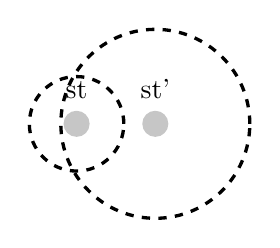
\begin{tikzpicture}
		\begin{scope}[very thick,dashed]
		\draw (0,1) circle (.6cm);
		\draw (0,1) node[circle,fill=gray!45,label=above:st]{};
		\draw (1,1) circle (1.2cm);t
		\draw (1,1) node[circle,fill=gray!45,label=above:st']{};
		\end{scope}
	\end{tikzpicture}
\end{figure}
		
\begin{figure}
    \caption{Link spoofing: Case 4} \label{chap3case4} 
    \centering
	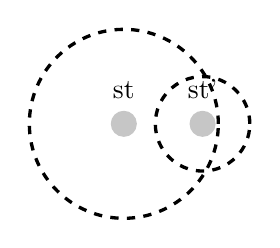
\begin{tikzpicture}
		\begin{scope}[very thick,dashed]
		\draw (0,1) circle (1.2cm);
		\draw (0,1) node[circle,fill=gray!45,label=above:st]{};
		\draw (1,1) circle (0.6cm);
		\draw (1,1) node[circle,fill=gray!45,label=above:st']{};
		\end{scope}
	\end{tikzpicture}

\end{figure}

<<<<<<< HEAD
\emph{Case 3}: $R_{st} \le dist(st,st')$ and $R_{st'} \ge dist(st,st')$. Let's call $\delta_d = dist(st,st') - R_{st}$, we calculate the message traveling time between $n$ and $n'$ as follows: 
\begin{equation*}
\begin{split}
		t(n') - t_n \ge \frac 1 {c}(dist(n,m) + dist(m', n')) + (t(m') - t(m)) \\ \Leftrightarrow
		t(n') - t_n \ge 2 \times \frac 1 {c}(dist(n,m)) + \delta_{tp}\\ \Leftrightarrow
		t(n') - t_n \ge 2 \times \frac 1 {c} (R_{st} + \delta_d) + \delta_{tp} \\ \Leftrightarrow
		2 \times \frac 1 {c} R_{st} + \delta_{tp} \ge 2 \times \frac 1 {c} (R_{st} + \delta_d ) + \delta_{tp} \\ \Leftrightarrow
		0 \ge \delta_{d} 
\end{split}
\end{equation*}
The only possible case is $\delta_{d}$ equals zero. It is too trivial. Otherwise, a fast relay attack occurs at the side from $st$ to $st'$. Case 3 is presented at figure~\ref{chap3case3}.

\emph{Case 4}: $R_{st} \ge dist(st,st')$ and $R_{st'} \le dist(st,st')$. This similarly happens as in case 3. If $R_{st}$ is much larger than $dist(st,st')$, then a fast relay attack occurs at the side from $st'$ to $st$. This is a undesirable result of time-based neighbour discovery protocols. Case 4, hence, is presented at figure~\ref{chap3case4}. $\qed$

=======
\emph{Case 3}: $R_{st} \le dist(st,st')$ and $R_{st'} \ge dist(st,st')$. Let's call $\Delta_d = dist(st,st') - R_{st}$, we calculate the message traveling time between $n$ and $n'$ as follows: 
\begin{equation*}
\begin{split}
		\tau_{n'} - \tau_{n} \ge \frac 1 {c}(dist(n,m) + dist(m', n')) + (\tau_{m'} - \tau_{m}) \\ \Leftrightarrow
		\tau_{n'} - \tau_{n} \ge 2 \times \frac 1 {c}(dist(n,m)) + \delta_{tp}\\ \Leftrightarrow
		\tau_{n'} - \tau_{n'} \ge 2 \times \frac 1 {c} (R_{st} + \Delta_d) + \delta_{tp} \\ \Leftrightarrow
		2 \times \frac 1 {c} R_{st} + \delta_{tp} \ge 2 \times \frac 1 {c} (R_{st} + \Delta_d ) + \delta_{tp} \\ \Leftrightarrow
		0 \ge \delta_{d} 
\end{split}
\end{equation*}
The only possible case is $\Delta_{d}$ equals zero. It is too trivial. Otherwise, a fast relay attack occurs at the side from $st$ to $st'$. Case 3 is presented at figure~\ref{chap3case3}.

\emph{Case 4}: $R_{st} \ge dist(st,st')$ and $R_{st'} \le dist(st,st')$. Presented at the figure~\ref{chap3case4}, it similarly happens as case 3. If $R_{st}$ is much larger than $dist(st,st')$, then a fast relay attack occurs at the side from $st'$ to $st$. 
>>>>>>> 3d6cc25ad869467a057daa522b35e3cad82b4604
%---------------------------Location-based-----------------------%
\subsubsection*{Location-based authentication test}

We formally describe location-based authentication test using knowledge of participant locations. 

\begin{Proposition}
<<<<<<< HEAD
Consider a weak penetrator model, and location information is confidentially exchanged and stored. Given strands $st, st' \in \mathcal{B}$, $\exists link(st,st', \leftrightarrow)$. If $|loc(st),loc(st')| \le R_{st}$, then $\exists plink(st, st',\leftrightarrow)$. 
=======
Consider a weak penetrator model, and location information is confidentially exchanged and stored. Given strands $st, st' \in \mathcal{B}$, $\exists link(st,st', \rightleftharpoons)$. If $|loc(st),loc(st')| \le R_{st}$, then $\exists plink(st, st',\rightleftharpoons)$. 
>>>>>>> 3d6cc25ad869467a057daa522b35e3cad82b4604
\end{Proposition}

\begin{proof}

Since $|loc(st),loc(st')| = dist(st,st')$, evidently $dist(st,st') \le R_{st}$. Furthermore, similarly to first part of proposition~\ref{samerange} proof, we infer $R_{st'} \ge R_{st}$. As a result, there exists a physical link between $st$ and st'. 

\end{proof}

Note that, without assumption on trusted location information, the location-based protocols may contain flaws in some cases. For instance, $st$ could not address correctly the physical location of $st'$ , then a penetrator use his knowledge about location of $st$ to make a fake link between them. Furthermore, location-based protocols share the same trouble with time-based protocols when analysed in our strong penetrator model. 

%-----------------------------------------------------------------------------------------------------------------------------------------------------------------------------%

\section{Analysis of ADVSIG}

<<<<<<< HEAD
In this section, we analyse ADVSIG protocol to show usefulness of our model. There are two kinds of strands in ADVSIG protocol:
\begin{enumerate}
\item Initiator strand $st = \{\langle st, 1 \rangle,\langle st, 2 \rangle,\langle st, 3 \rangle,\langle st, 4 \rangle\} \\ \in Init[A,t_1,t_3,ASYM\_LINK, SYM\_LINK]$ with trace $<+M_1, -M_2 , +M_3,-M_4>$
\item Responder strand $st' = \{\langle st', 1 \rangle,\langle st', 2 \rangle,\langle st', 3 \rangle,\langle st', 4 \rangle\} \\ \in Resp[B,t_2,t_4,ASYM\_LINK, SYM\_LINK]$ with trace $<-M_1, +M_2 , -M_3,+M_4>$
=======
ADVSIG proposed by INRIA group~\cite{Raffo:2004:ASS:1029102.1029106} is a kind of secure routing protocol fortifying for OLSR \cite{Clausen:2003:OLS:RFC3626}. In this protocol, a node wishes to detect neighbours with bi-directional physical links. The protocol is presented as below. 
\begin{flushleft}
 \emph{M1:} $A \to [B]: \{\O, \O, \tau_0\}_{KA}$\\
 \emph{M2:} $B \to [A]: \{\{"A:ASYM\_LINK", \tau_1\}_{KB}, \O,\tau_1\}_{KB}$\\
\emph{M3:} $A \to [B]: \{\{"B:ASYM\_LINK",\tau_2\}_{KA},\O ,\tau_2 \}_{KA})$\\
 \emph{M4:} $B \to [A] : \{\{"A:SYM\_LINK", \tau_3\}_{KB} ,\{"B:ASYM\_LINK",\tau_2\}_{KA} ,\tau_3\}_{KB})$
\end{flushleft}

Moreover, every valid link state must satisfy a maximum interval $\delta_{max}$ defined by $|T_{Sender} - T_e | < \delta_{max}$ where $T_{Sender}$ is the value clock of the sender, and $T_e$ is the value clock of receiver. 

Provided that the third message does not include the proof from the second one, Responder cannot ensure if Initiator has been received the second message or not. As the result of that, internal attackers can produce the first and third messages to valid a protocol run with Responder. Additionally,  neighbours of Responder could be impacted by this attack due to two-hop sensing mechanism in the OLSR protocol.  Figure~\ref{advsigattack3} outlines an attacking scenario to ADVSIG where there only appears a unidirectional link X $\rightarrow$ B.

In the attack scenario, we assume that $X$ accidentally knows the existence of $B$ out of $X$'s physical signal coverage. By using a high power antenna, $X$ can enlarge its signal range. Then $X$ emits valid messages $M1$ and $M3$ to $B$, this makes $B$ believe a existence of bidirectional link between $B$ and $X$.   

\begin{figure}
		\caption{ADVSIG Attack }\label{advsigattack3}
        \centering
        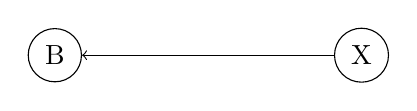
\begin{tikzpicture}
		\draw [<-](1,1) node[anchor=east,circle,draw]{B} to (4.2,1) node[anchor=west,circle,draw]{X};
		\end{tikzpicture}

	    \centering
        \begin{tikzpicture}[implies/.style={double,double equal sign distance,-implies},
  			dot/.style={shape=circle,fill=black,minimum size=2pt,
  		      inner sep=0pt,outer sep=2pt},thick,scale=0.8, every node/.style={scale=0.8}]
		\matrix[matrix of nodes] {
		  |[dot,label=above:$B$] (B1)| {} & [2cm]|[] (C1)| {}&[1cm] |[dot,label=above:$X$] (X1)| {}\\[1cm]
  		  |[dot] (B2)| {} & [2cm]|[dot,label=above:$*$] (C2)| {}& [1cm]|[dot] (X2)| {}\\[1cm]
  	      |[dot] (B3)| {} & [2cm]|[] (C3)| {}& [2cm]|[dot] (X3)| {}\\[1cm]
 		  |[dot] (B4)| {} & [2cm]|[dot,label=above:$*$] (C4)| {}& [1cm]|[] (X4)| {}\\
		};
		\draw (X1) edge[->] node[above] {M1} (B1)
	      edge[implies] (X3); 
		\draw (B2) edge[->] node[above] {M2} (C2)
	      edge[implies,implies-] (B1);
		\draw (B3) edge[<-] node[above] {M3} (X3)
    	  edge[implies,implies-] (B2);
		\draw (B4) edge[->] node[above] {M4} (C4)
    	  edge[implies,implies-] (B3);
		\end{tikzpicture}

\end{figure}

We analyse ADVSIG protocol to show usefulness of our model. There are two kinds of strands in ADVSIG protocol:
\begin{enumerate}
\item Initiator strand $st =  \{\langle st, 1 \rangle,\langle st, 2 \rangle,\langle st, 3 \rangle,\langle st, 4 \rangle\}\\ \in Init[A,\tau_1,\tau_3]$ with trace $<+M_1, -M_2 , +M_3,-M_4>$
\item Responder strand $st' = \{\langle st', 1 \rangle,\langle st', 2 \rangle,\langle st', 3 \rangle,\langle st', 4 \rangle\} \\ \in Resp[B,\tau_2,\tau_4]$ with trace $<-M_1, +M_2 , -M_3,+M_4>$
>>>>>>> 3d6cc25ad869467a057daa522b35e3cad82b4604
\end{enumerate}

Protocol assumption: 
\begin{itemize}
\item ps1: $|T_{sender} - T_e| < \delta_{max}$
\item ps2: Time synchronisation mechanism is set on participants.
\end{itemize}

\subsubsection*{Initiator's Guarantee} 

The initiator states the guarantee as follows.

<<<<<<< HEAD
Suppose $\mathcal{B}$ is a wireless bundle. Under the conditions $ps1, ps2$, if $\mathcal{B}$ contains a strand $st \in Init[A,t_1,t_3,ASYM\_LINK, SYM\_LINK]$ with $\mathcal{B} -height$ 4, then $\mathcal{B}$ contains a strand $st' \in Resp[B,t_2,t_4,ASYM\_LINK, SYM\_LINK]$ with $\mathcal{B} -height$ 4, and there exists a $plink(st,st',\leftrightarrow)$. 

Mechanically, to find out if the statement is correct or not, we start asserting the logical link guarantee between two participants. 
 
\emph{Logical link guarantee}: At first, we search for a DE edge with an identification factor:
\begin{itemize}
\item The edge $\langle st, 1 \rangle \Rightarrow \langle st, 2 \rangle$ does not contain any identification factor in the challenge message. 
\item The edge $\langle st, 3 \rangle \Rightarrow \langle st, 4 \rangle$ : $term(\langle st, 3 \rangle)$ contains a clear-form identification factor which is response's name $B$ and a timestamp $t_2$, all signed by A's private key, and $term(\langle st, 4 \rangle)$ embodies the a clear-form provable component $\{\{ "A:SYM\_LINK", t_3\}_{KB} ,\{ "B:ASYM\_LINK",t_2\}_{KA} ,t_3\}_{KB}$.
\end{itemize}

The edge $\langle st, 3 \rangle \Rightarrow \langle st, 4 \rangle$ satisfies the authentication logical link test. Therefore, A can verify a logical link between A and B, and B is a regular party. To find out if there exists $plink(st,st,\leftrightarrow)$, we apply the time-based authentication test. 

\emph{Physical link guarantee}: To verify the distance between $st$ and $st'$, we apply the time-based authentication test for the edge $\langle st, 3 \rangle \Rightarrow \langle st, 4 \rangle$. The test concludes that if $(t(\langle st, 4 \rangle) - t(\langle st, 3 \rangle)) \div 2 \le R_{st} \div c$ + $\delta_{tp} \div 2$ (1) then $\exists plink(st,st', \leftrightarrow)$. 

Basing on assumption ps1 and ps2, we calculate the message traveling time from node $\langle st, 3 \rangle$ to $\langle st, 4 \rangle$:
\begin{equation*}
\label{equation1}
\begin{split}
t(\langle st,4\rangle) - t(\langle st, 3 \rangle) = \\
(t(\langle st', 3 \rangle) - t(\langle st, 3 \rangle)) + \\
(t(\langle st', 4 \rangle) - t(\langle st', 3 \rangle)) + \\
(t(\langle st, 4 \rangle) - t(\langle st', 4 \rangle)) \\
\Rightarrow t(\langle st,4\rangle) - t(\langle st, 3 \rangle) \le 2 \times \delta_{max} + \delta_{tp} (2)
=======
Suppose $\mathcal{B}$ is a wireless bundle. Under the conditions $ps1, ps2$, if $\mathcal{B}$ contains a strand $st \in Init[A,\tau_1,\tau_3]$ with $\mathcal{B} -height$ 4, then $\mathcal{B}$ contains a strand $st' \in Resp[B,\tau_2,\tau_4]$ with $\mathcal{B} -height$ 4, and there exists a $plink(st,st',\rightleftharpoons)$. 

Mechanically, to find out if the statement is correct or not, we start asserting the logical link guarantee between two participants. Let's call node $n_1$,  $n_2$, $n_3$ and $n_4$ be $\langle st,1\rangle$, $\langle st,2\rangle$, $\langle st,3\rangle$, and $\langle st,4\rangle$ respectively. 
 
\emph{Logical link guarantee}: At first, we search for a DE edge with an identification factor:
\begin{itemize}
\item The edge $n_1 \Rightarrow n_2$ does not contain any identification factor in the challenge message. 
\item The edge $n_3 \Rightarrow n_4$ : $term(n_3)$ contains a clear-form identification factor which is response's name $B$ and a timestamp $\tau_2$, all signed by A's private key, and $term(n_4)$ embodies the a clear-form provable component $\{\{ "A:SYM\_LINK", \tau_3\}_{KB} ,\{ "B:ASYM\_LINK",\tau_2\}_{KA} ,\tau_3\}_{KB}$.
\end{itemize}

The edge $n_3 \Rightarrow n_4$ satisfies the authentication logical link test. Therefore, $A$ can verify a logical link between $A$ and $B$, and $B$ is a regular party. To find out if there exists $plink(st,st,\rightleftharpoons)$, we apply the time-based authentication test.  

\emph{Physical link guarantee}: To verify the distance between $st$ and $st'$, we apply the time-based authentication test for the edge $n_3 \Rightarrow n_4$. The test concludes that if $(t_{n_4} - t_{n_3}) \div 2 \le R_{st} \div c$ + $\delta_{tp} \div 2$ (1) then $\exists plink(st,st', \rightleftharpoons)$. Let's call node $n'_3$ and $n'_4$ be $\langle st',3\rangle$, and $\langle st',4\rangle$ respectively. 

Basing on assumption ps1 and ps2, we calculate the message traveling time from node $n_3$ to $n_4$:
\begin{equation*}
\label{equation1}
\begin{split}
t_{n_4} - t_{n_3} = \\
(t_{n'_3} - t_{n_3}) + (t_{n'_4} - t_{n'_3}) + (t_{n_4} - t_{n'_4}) \\
\Rightarrow t_{n_4} - t_{n_3} \le 2 \times \delta_{max} + \delta_{tp} (2)
>>>>>>> 3d6cc25ad869467a057daa522b35e3cad82b4604
\end{split}
\end{equation*}

 Let $2\times(1) - (2)$, we have
\begin{equation*}
\label{equation2}
\begin{split}
	R_{st} \div c - \delta_{max} \ge 0 (3)
\end{split}
\end{equation*}

<<<<<<< HEAD
If inequality (3) holds, then $\exists plink(st,st', \leftrightarrow)$. $\qed$
=======
If inequality (3) holds, then $\exists plink(st,st', \rightleftharpoons)$. $\qed$
>>>>>>> 3d6cc25ad869467a057daa522b35e3cad82b4604
  
\subsubsection*{Responders Guarantee}

The initiator states the guarantee as follows.

<<<<<<< HEAD
Suppose $\mathcal{B}$ is a wireless bundle. Under the conditions $ps1, ps2$, if $\mathcal{B}$ contains a strand $st' \in Resp[A,t_1,t_3,ASYM\_LINK, SYM\_LINK]$ with $\mathcal{B} -height$ 4, then $\mathcal{B}$ contains a strand $st \in Init[B,t_2,t_4,ASYM\_LINK, SYM\_LINK]$ with $\mathcal{B} -height$ 4, and there exists a $plink(st,st',\leftrightarrow)$. 

The proof of this statement is quite identical to initiator's guarantee. However, when looking for a double logical link, regrettably, we cannot find any logical link test edge in the responder strand. As a result, $B$ can be a victim of spoofing attack. $\qed$ 
 
\subsubsection*{Link spoofing attack on ADVSIG} 

Formally describing, let's call node $n_1$ and $n_2$ be $\langle st, 1 \rangle$ and $\langle st, 3 \rangle$ respectively. Since $n_1$ and $n_3$ do not contain any proof of reception, they possibly lie on B strand. Definitely, they do. 

When X accidentally knows the existence of B but it cannot listen to B, X persuades B that B will own a double physical link with X. Thus, penetrator X strand is: 
\begin{center}
$st_x =$ $\{(M_1,loc(\langle st_X,1\rangle),t(\langle st_X,1\rangle), R_M),(M_3,loc(\langle st_X,2\rangle),t(\langle st_X,2\rangle), R_M)\}$ $\in$ \\
$Init[X,t_1,t_2,t_3,ASYM\_LINK,SYM\_LINK]$ with trace $<+M_1,+M_3>$.
\end{center}
=======
Suppose $\mathcal{B}$ is a wireless bundle. Under the conditions $ps1, ps2$, if $\mathcal{B}$ contains a strand $st' \in Resp[A,\tau_1,\tau_3]$ with $\mathcal{B} -height$ 4, then $\mathcal{B}$ contains a strand $st \in Init[B,\tau_2,\tau_4]$ with $\mathcal{B} -height$ 4, and there exists a $plink(st,st',\rightleftharpoons)$. 

The proof of this statement is quite identical to initiator's guarantee. However, when looking for a bidirectional logical link, regrettably, we cannot find any logical link test edge in the responder strand. As a result, $B$ can be a victim of spoofing attack. $\qed$ 
 
\subsubsection*{Link spoofing attack on ADVSIG} 

Since $n_1$ and $n_3$ do not contain any proof of reception, they possibly lie on $X$ strand. Definitely, they do. 

When $X$ accidentally knows the existence of $B$ but it cannot listen to $B$, $X$ persuades $B$ that $B$ will own a bidirectional physical link with X. Thus, penetrator X strand is: 
\begin{flushleft}
$st_x = \{(M_1,loc(\langle st_X,1\rangle),\tau_{x1}, R_M) ,(M_3,loc(\langle st_X,2\rangle)$ \\ $,\tau_{x3}, R_M)\}$ $\in$ 
 $Init[X,\tau_{x1},\tau_{2},\tau_{x3}]$ with trace $<+M_1,+M_3>$.
\end{flushleft}

Furthermore, we found a similar flaw in the work~\cite{Adnane20131159}. The authors proposed a trusted-based security for OLSR protocols where all participants must trust together. However, internal attackers can successfully create a fake bidirectional physical link to a target as they do in ADVSIG. 
>>>>>>> 3d6cc25ad869467a057daa522b35e3cad82b4604

\section{Conclusion}

This chapter has addressed a serious problem of current neighbour discovery protocols that have not introduced before. The problem comes when participants use wireless interfaces with different signal power, that leads the ND protocols cannot correctly verify the distance between participants.  

We extended the original strand space model to be able to analyse secure neighbour protocols. To achieve this, we modified the model so that it becomes possible to take into account some physical properties including timestamp, location, and signal propagation. The penetrator model has been adapted in consequence. Thank our model, time-based, even location-based neighbour discovery techniques were formally proved that they would not guarantee the existence of physical bidirectional links. 

Aforementioned works on this topic, mainly apply existing verification tools initially. We rather chosen to define a dedicated formalism able to model physical properties in neighbour discovery protocols in a natural manner, and the results obtained so far seems promising. Concerning future work, we will first try to extend the model in order to capture mobility and network topology. In a second step, we plan to study how we could automate the analysis procedure.
